\documentclass[10pt]{exam}
\usepackage[hon]{template-for-exam}
\usepackage{endnotes,graphicx}
\usepackage{tikz,graphicx,enumitem,multicol,float,my-tikz-clipart,silence,cclicenses}
\graphicspath{{./figures/}}
\WarningFilter{latex}{Label `part}
\WarningFilter{latex}{There were multiply-defined labels}

\footer{}{\thepage}{\sc \myclass}


%\def\answer#1{\footnotetext{#1}}
%\def\myquestion{\item\stepcounter{footnote}}

\def\enoteheading{}
\def\answer#1{\endnotetext{#1}}
\def\theanswers{\theendnotes}
\def\myquestion{\item\stepcounter{endnote}}

\newenvironment{myquestions}{
  \begin{multicols}{2}\begin{enumerate}[resume]
}{
  \end{enumerate}\end{multicols}
}
\makeatletter
\patchcmd{\enit@setresumekeys}{\def}{\gdef}{}{}
\patchcmd{\enit@setresumekeys}{\def}{\gdef}{}{}
\makeatother

\newcommand{\myheading}[1]{\uplevel{\section*{#1}}
}
\newcommand{\mysubheading}[1]{\uplevel{\subsection*{#1}}
}

%uncomment if running Pandoc
% \renewcommand{\myheading}[1]{{\section*{#1}}}
% \renewcommand{\mysubheading}[1]{\subsection*{#1}}


\def\HWDue{Mon, Apr 27}
\def\TestDay{Fri, May 8}


\def\mytitle{Chapter 18 HW (Electrostatics)}
\title{\mytitle}
\date{\today}

\def\mymaketitle{
  \begin{flushleft}
    {\LARGE \textbf \mytitle \par}
  \end{flushleft}
}

\newcommand{\bs}[2]{\textbf{#1} (\sc #2 Points)}


\newcommand{\GFig}[3]{  
  \begin{figure}[H]
    \centering
    \includegraphics[width=#3]{#1_#2_Figure.jpg}
    \caption{Giancolli Figure #1-#2.}
    \label{#1-#2}
  \end{figure}
}


\begin{document}
\maketitle
% \begin{center}
%   
\includegraphics[width=10cm]{sound-wave.png}
% \end{center}

\noindent
This HW packet is due on \textbf{\HWDue}.  There will also be a Circuits assignment that is due on Test Day, \textbf{\TestDay}.

\vspace{1em}
\hrule

\vspace{1em}
\noindent
Questions and figures are from OpenStax \emph{College Physics}, 2e (Chapter 18) or Giancolli \emph{Physics: Principles with Applications}, 7th ed, (Chapter 16) unless otherwise noted.


\section*{Coulomb's Law Concepts}


\begin{enumerate}[resume]


\myquestion (CQ2)
  Why do most objects tend to contain nearly equal numbers of positive and negative charges? \vs

% \myquestion (CQ8)
%   What is grounding? What effect does it have on a charged conductor? On a charged insulator? \vs

\myquestion (P12) \answer{0.56 N}
  Two point charges exert a 5.00 N force on each other. What will the force become if the distance between them is increased by a factor of three? \vs

\myquestion (P13) \answer{factor of 5}
  Two point charges are brought closer together, increasing the force between them by a factor of 25. By what factor was their separation decreased? \vs

\myquestion (Giancoli CQ10)
  The form of Coulomb's law is very similar to that for Newton's law of universal gravitation. What are the differences between these two laws? Compare also gravitational mass and electric charge. \vs

\myquestion (Giancoli MCQ3) \answer{they are attracted to each other equally}
  Fred the lightning bug has a mass m and a charge $+q$. Jane, his lightning-bug wife, has a mass of $43m$ and a charge $-2q$. Because they have charges of opposite sign, they are attracted to each other. Which is attracted more to the other, and by how much? \vs

\myquestion (Giancoli MCQ6) \answer{mass decreases}
  As an object acquires a positive charge, does its mass usually increase, decrease, or stay the same? Why? \vs



\end{enumerate}

\pagebreak

\section*{Coulomb's Law Problems}

\begin{myquestions}
\myquestion (P1) \answer{(a) \SI{1.25e10}{}; 
(b) \SI{3.13e12}{}}
  Common static electricity involves charges ranging from nanocoulombs to microcoulombs. (a) How many electrons are needed to form a charge of \SI{-2.00}{nC}?  (b) How many electrons must be removed from a neutral object to leave a net charge of \SI{0.500}{\micro C}?
\myquestion (P10) \answer{\SI{1.27e-3}{N}} 
  What is the repulsive force between two pith balls that are 8.00 cm apart and have equal charges of  $-30.0$~nC?
\myquestion (Giancoli P11) \answer{115.8 N, left; 564.2 N, right; 448.4 N, left}
  Particles of charge $+\SI{65}{\micro C}$, $+\SI{48}{\micro C}$, and $-\SI{95}{\micro C}$ and are placed in a line (Figure~\ref{16-52}). The center one is 35~cm from each of the others. Calculate the net force on each charge due to the other two.
  %
  \GFig{16}{52}{6cm}

\uplevel{Additional Practice: \#\ref{coulomb-i}-\ref{coulomb-f}}
\end{myquestions}

\pagebreak

\section*{Electric Field Concepts}

\begin{myquestions}
\myquestion (P33) 
  (a) Sketch the electric field lines near a point charge +q. (b) Do the same for a point charge -3.00q.
  \vs \columnbreak

\myquestion (P34a) \answer{$q_2=q_1/2$}
Figure~\ref{18.43} shows the electric field lines near two charges $q_1$ and $q_2$. What is the ratio of their magnitudes?
  %
  \begin{figure}[H]
    \centering
    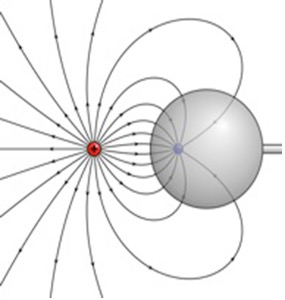
\includegraphics[width=6cm]{18-43.jpg}
    \caption{OpenStax Figure 18.43. The electric field near two charges.}
    \label{18.43}
  \end{figure}
\end{myquestions}

\vs

\hrule

\begin{myquestions}
\myquestion (Giancoli Q14)
  When determining an electric field, must we use a positive test charge, or would a negative one do as well? Explain.
  \vs \columnbreak

\myquestion (Giancoli MCQ12) \answer{(d)}
  Which vector best represents the direction of the electric field at the fourth corner of the square due to the three charges shown in Figure~\ref{16-51}?  Explain.
  %
  \GFig{16}{51}{4cm}

\end{myquestions}

\vs

\pagebreak

\section*{Electric Field Problems}

\begin{myquestions}
  
\myquestion (P29) \answer{\SI{1.12e7}{N/C}}
  Calculate the magnitude of the electric field 2.00~m from a point charge of 5.00~mC (such as found on the terminal of a Van de Graaff).
  
\myquestion (P27) \answer{\SI{-11.4}{N/C}, downward}
  What is the magnitude and direction of an electric field that exerts a \SI{2.00e-5}{N} upward force on a \SI{-1.75}{\micro C} charge?

\vspace*{\stretch{1}}


\myquestion (P28) \answer{\SI{8.75e-4}{N}}
  What is the magnitude and direction of the force exerted on a \SI{3.50}{\micro C} charge by a \SI{250}{N/C} electric field that points due east?

\myquestion (P42b) \answer{\SI{2.03e5}{N/C}}
  Find the total electric field at $x=11.00$~cm in Figure~\ref{18.48} given that $q=5.00$~nC. 


\uplevel{Additional Practice: \#\ref{field-i}-\ref{field-f}}
  

\end{myquestions}

  \begin{figure}[H]
    \centering
    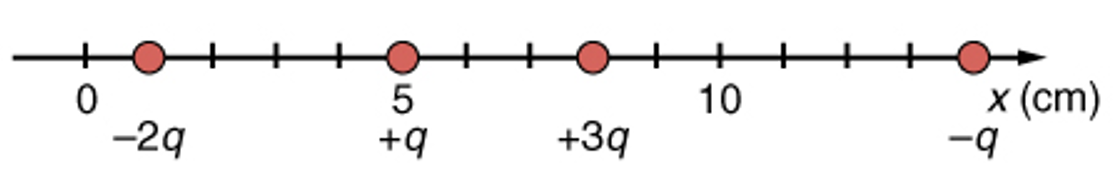
\includegraphics[width=9cm]{18-48b.png}
    \caption{OpenStax Figure 18.48(b). Point charges located at 1.00, 5.00, 8.00, and 14.0 cm along the $x$-axis.  [Assume that $q=\SI{5.00}{nC}$.]}
    \label{18.48}
  \end{figure}


\pagebreak

\section*{Electric Potential Problems}

\begin{myquestions}

\myquestion (Giancoli Ch 17 P1) \answer{\SI{5.0e-4}{J}}
  How much work does the electric field do in moving a charge of magnitude \SI{-7.7}{\micro C} from ground to a point whose potential is $+65$~V higher?

\myquestion (Giancoli Ch 17 P2) \answer{\SI{2.72e-17}{J}}
  How much work does the electric field do in moving a proton from a point at a potential of $+125$~V to a point at $-45$~V?
\end{myquestions}

\vs

\section*{Electric Potential Concept}

\begin{enumerate}[resume]
\myquestion (Giancoli Ch 17 CQ2) \answer{negative will move toward higher potential}
  If a negative charge is initially at rest in an electric field, will it move toward a region of higher potential or lower potential? What about a positive charge? \vspace{10em}
\end{enumerate}



\pagebreak


\begin{myquestions}

\myheading{Additional Practice}


\myquestion (P14) \answer{7.11 mm} \label{coulomb-i}
  How far apart must two point charges of 75.0~nC (typical of static electricity) be to have a force of 1.00 N between them?

\myquestion (P15) \answer{\SI{9e3}{N}}
  If two equal charges each of 1 C each are separated in air by a distance of 1 km, what is the magnitude of the force acting between them? You will see that even at a distance as large as 1 km, the repulsive force is substantial because 1 C is a very significant amount of charge. 

\myquestion (P16) \answer{10 N, away from \SI{6}{\micro C}} \label{coulomb-f}
  A test charge of $+\SI{2}{\micro C}$ is placed halfway between a charge of $+\SI{6}{\micro C}$  and another of $+\SI{4}{\micro C}$ separated by 10~cm. (a) What is the magnitude of the force on the test charge? (b) What is the direction of this force (away from or toward the $+\SI{6}{\micro C}$ charge)?

\myquestion (P32) \answer{(a) 300 N/C, east; (b) \SI{4.80e-17}{N}, east} \label{field-i}
  (a) Find the magnitude and direction of an electric field that exerts a \SI{4.80e-17}{N} westward force on an electron. (b) What magnitude and direction force does this field exert on a proton?

\myquestion (Giancoli P24) \answer{\SI{3.45e7}{N/C}} \label{field-f}
  Determine the magnitude and direction of the electric field at a point midway between a $-\SI{8.0}{\micro C}$ and a $+\SI{5.8}{\micro C}$ charge 6.0~cm apart. Assume no other charges are nearby.


\myheading{Bonus}


\myquestion (Giancoli P15)
  At each corner of a square of side $l$ there are point charges of magnitude $Q$, $2Q$, $3Q$, and $4Q$ (Figure~\ref{16-54}). Determine the magnitude and direction of the force on the charge $2Q$.
  %
  \GFig{16}{54}{2.7cm}


\myquestion (P60) \answer{\SI{6890}{N/C}}
  \textbf{Integrated Concepts.} A 5.00-g charged insulating ball hangs on a 30.0 cm long string in a uniform horizontal electric field as shown in Figure~\ref{18.52}. Given the charge on the ball is \SI{1.00}{\micro C}, find the strength of the field%
  %
  \begin{figure}[H]
    \centering
    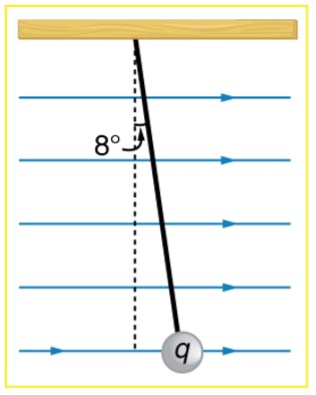
\includegraphics[width=2.8cm]{18-52.jpg}
    \caption{OpenStax Figure 18.52.  A horizontal electric field causes the charged ball to hang at an angle of $8.00^\circ$.}
    \label{18.52}
  \end{figure}
  
\myquestion (P62) \answer{(a) \SI{3.78e-14}{N}; (b) \SI{-2.36e5}{N/C}}
	\textbf{Integrated Concepts.} The classic Millikan oil drop experiment was the first to obtain an accurate measurement of the charge on an electron. In it, oil drops were suspended against the gravitational force by a vertical electric field. (See Figure~\ref{18.54}.) Given the oil drop to be \SI{1.00}{\micro m}  in radius and have a density of \SI{920}{kg/m^3}: (a) Find the weight of the drop. (b) If the drop has a single excess electron, find the electric field strength needed to balance its weight.
  %
  \begin{figure}[H]
    \centering
    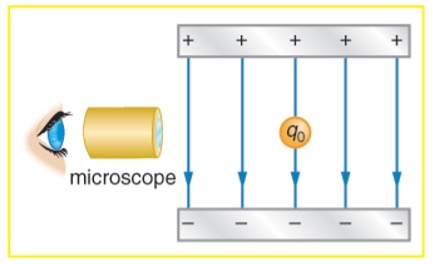
\includegraphics[width=6cm]{18-54.jpg}
    \caption{OpenStax Figure  18.54.  In the Millikan oil drop experiment, small drops can be suspended in an electric field by the force exerted on a single excess electron. Classically, this experiment was used to determine the electron charge $e$  by measuring the electric field and mass of the drop.}
    \label{18.54}
  \end{figure}
  


\end{myquestions}

\pagebreak


\section*{Equations}

\subsection*{Electrostatics Equations}

\begin{align*}
  F &= \frac{kq_1 q_2} {r^2} &
  E &\equiv \frac{F}{q} = \frac{kq}{r^2} &
  \Delta V &= -\frac{W}{q}
\end{align*}

\subsection*{Circuits Equations}

\begin{align*}
  I &\equiv \frac{\Delta q}{\Delta t} &
  \Delta V &= IR &
  P &= I\Delta V = I^2 R = \frac{\Delta V^2}{R}
\end{align*}


\begin{align*}
  R_{eq} &= R_1 + R_2 + \cdots &
  \frac{1}{R_{eq}} &= \frac{1}{R_1} + \frac{1}{R_2} + \vdots
\end{align*}

\subsection*{Unit Conversions}

\begin{align*}
  \SI{1}{mC} &= \SI{e-3}{C} &
  \SI{1}{\micro C} &= \SI{e-6}{C} &
  \SI{1}{n C} &= \SI{e-9}{C}
\end{align*}


\subsection*{Constants}

\vspace{2em}

\begin{tabular}{ll}
Coulomb Constant          &   $k = \SI{9.0e9}{\newton\meter^2\per\coulomb^2}$\\
Charge of electron/proton &   $e=\pm\SI{1.60e-19}{\coulomb}$\\
Electron mass             &   $m_e=\SI{9.11e-31}{\kilo\gram}$\\
Proton mass	              &   $m_p=\SI{1.673e-27}{\kilo\gram}$\\
Neutron mass	            &   $m_n=\SI{1.675e-27}{\kilo\gram}$
\end{tabular}

\vs
\hrule

\section*{Selected Answers}

  \renewcommand{\enotesize}{\normalsize}
  \renewcommand{\enoteformat}{%
    \leftskip=1.8em
    \makebox[0pt][r]{\theenmark. }%
  }

  \hfill

  \begin{multicols}{2}
    \theanswers
  \end{multicols}
  \pagebreak

  (scratch work)


\end{document}